%%%% compile with
%%% latexmk -auxdir=aux/ main.tex
\documentclass{irdbeamer}
\usepackage{tikz}
\usepackage{pgfplots}
\usepackage{animate}

\title{Sampling and overfitting}
\subtitle{Formation IA biodiversité}
\author[Paul Tresson]{Paul Tresson}
\date{\today} % or whatever the date you are presenting in is
\institute[Institut de Recherche pour le Développement]{UMR AMAP}

%\copyrightnotice{Published by Institut de Recherche pour le Développement, with permission}

% %% to add a background image for the title slide, uncomment here
% \usebackgroundtemplate{
%   \tikz[overlay, remember picture] \node[at=(current page.center)] {
%     \includegraphics[width=\paperwidth,height=\paperheight]{example-image-a}
%   };
% }

\usepackage[
    backend=biber,
    style=authoryear-comp,
    maxcitenames=2, % max 2 authors before switching to et al.
    maxbibnames=4,
    uniquelist=false, % stays et al. when almost the same authors
    uniquename=false, % dose not bother when first name not written the same way everywhere
    date=year, % month does not appear in bibliography
    natbib=true, % use natbib synthax
    url=false, % remove url
    eprint=false % remove eprint
]{biblatex}

\addbibresource{refs.bib}

\let\oldcite=\cite                                                              
\renewcommand{\cite}[1]{\textcolor[rgb]{.5,.5,.7}{\oldcite{#1}}}
\let\oldcitep=\citep                                                              
\renewcommand{\citep}[1]{\textcolor[rgb]{.5,.5,.7}{\oldcitep{#1}}}

\begin{document}

\addlogo{logos/IRD_banner.png}
\addlogo{logos/AMAP_banner.png}
\maketitle

\usebackgroundtemplate{}

\section{Introduction}

\begin{frame}{What do we want when modelling ?}
    
\end{frame}

\begin{frame}{What do we want when modelling ?}
    
    All models are wrong but some are useful
\end{frame}

\section{Overfitting}

\begin{frame}{What is overfitting}
    \centering
    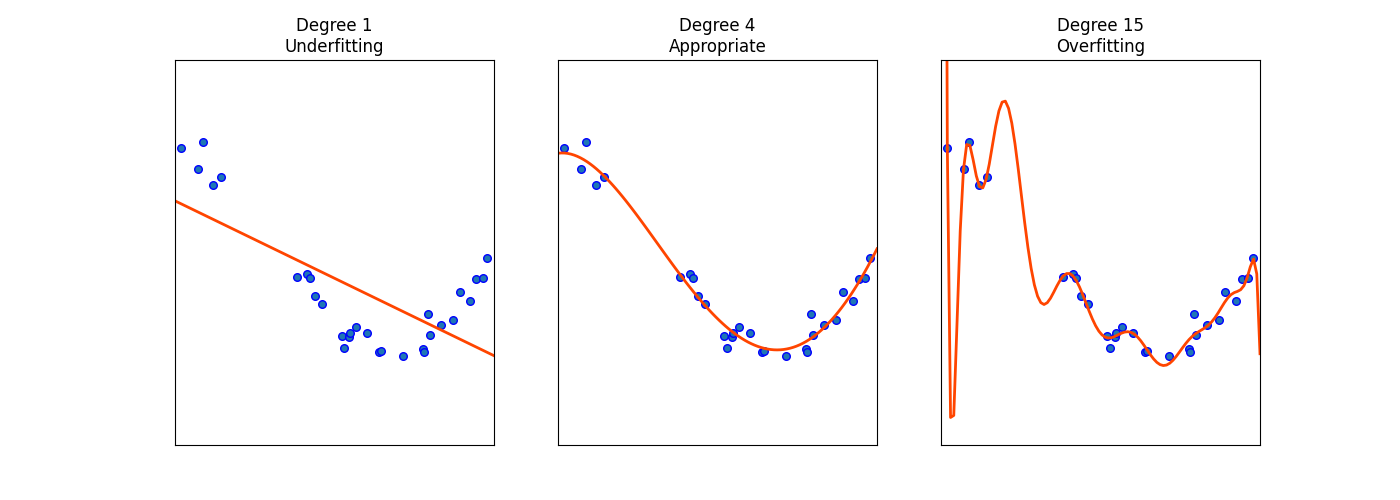
\includegraphics[width = .8\textwidth]{./figs/overfitting-overview.png}
    \nonumbernote{\tiny adapted from scikit-learn docs}
\end{frame}

\begin{frame}{Common tools and intuitions - Train/Test loss}
    \begin{columns}
        \begin{column}{.5\linewidth}
    \centering
    \vspace{1cm}
    \includegraphics<1>[width = .8\textwidth]{./figs/plot/overfitting1.png}%
    \includegraphics<2>[width = .8\textwidth]{./figs/plot/overfitting2.png}%
    \includegraphics<3>[width = .8\textwidth]{./figs/plot/overfitting3.png}%
    \includegraphics<4>[width = .8\textwidth]{./figs/plot/overfitting4.png}%
    \includegraphics<5>[width = .8\textwidth]{./figs/plot/overfitting5.png}%
    \includegraphics<6>[width = .8\textwidth]{./figs/plot/overfitting6.png}%
    \includegraphics<7>[width = .8\textwidth]{./figs/plot/overfitting7.png}%
    \includegraphics<8>[width = .8\textwidth]{./figs/plot/overfitting8.png}%
    \includegraphics<9>[width = .8\textwidth]{./figs/plot/overfitting9.png}%
        \end{column}
        \begin{column}{.5\linewidth}
    \centering
    \includegraphics<1>[width = .8\textwidth]{./figs/plot/train_test_loss-1.png}%
    \includegraphics<2>[width = .8\textwidth]{./figs/plot/train_test_loss-2.png}%
    \includegraphics<3>[width = .8\textwidth]{./figs/plot/train_test_loss-3.png}%
    \includegraphics<4>[width = .8\textwidth]{./figs/plot/train_test_loss-4.png}%
    \includegraphics<5>[width = .8\textwidth]{./figs/plot/train_test_loss-5.png}%
    \includegraphics<6>[width = .8\textwidth]{./figs/plot/train_test_loss-6.png}%
    \includegraphics<7>[width = .8\textwidth]{./figs/plot/train_test_loss-7.png}%
    \includegraphics<8>[width = .8\textwidth]{./figs/plot/train_test_loss-8.png}%
    \includegraphics<9>[width = .8\textwidth]{./figs/plot/train_test_loss-9.png}%
        \end{column}
    \end{columns}
\end{frame}

\begin{frame}{Common tools and intuitions - Train/Test loss}
    \begin{figure}
        \centering
        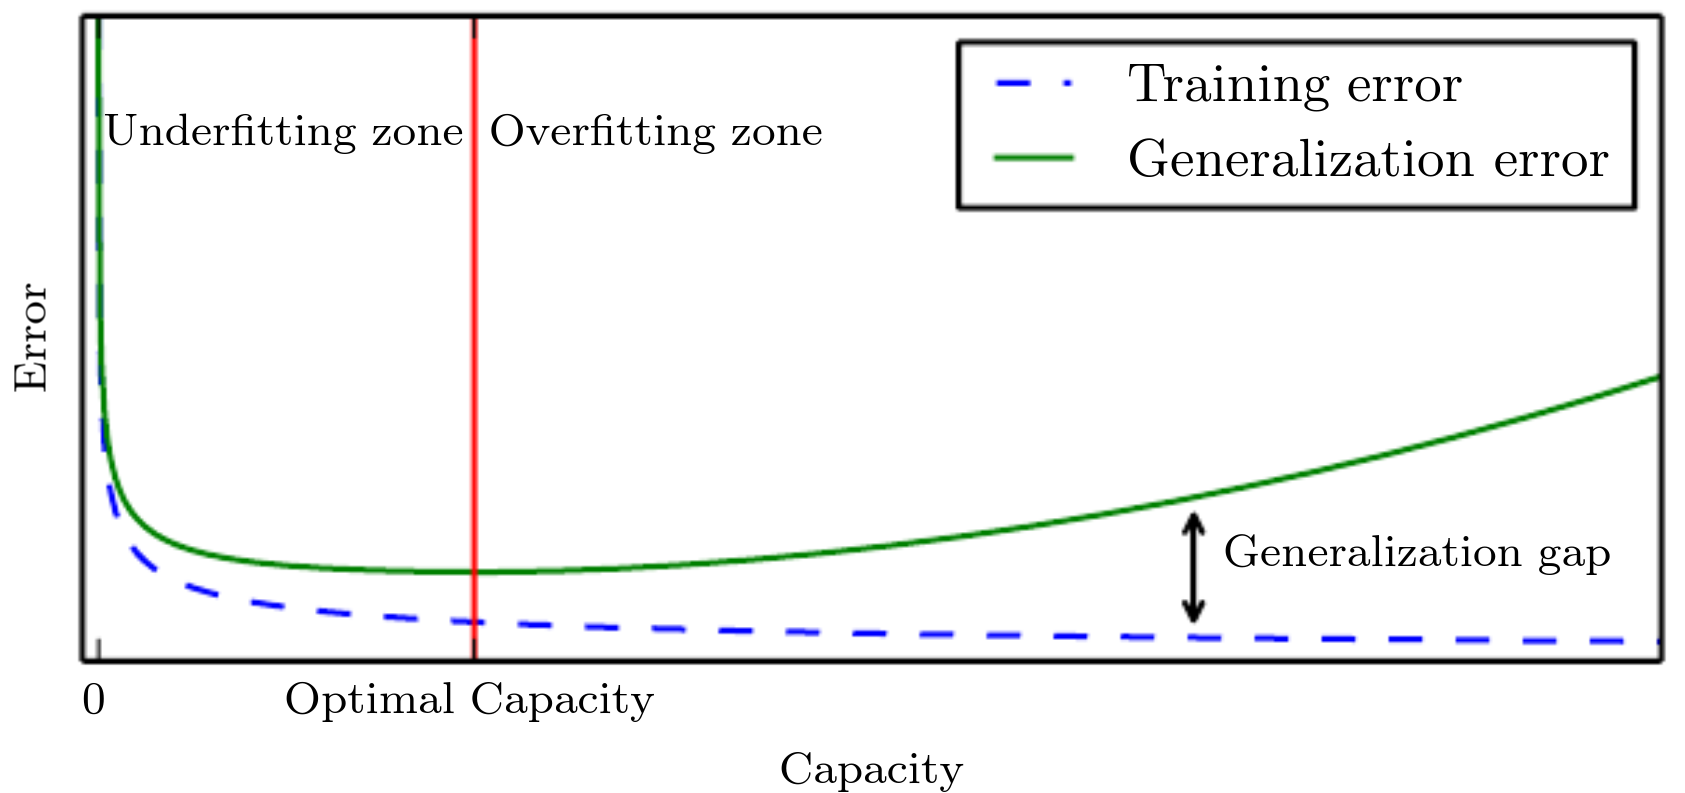
\includegraphics[width = .8\textwidth]{./figs/goodfellow.png}
        \caption{\tiny Figure from \cite{goodfellow2016deep}}
    \end{figure}
\end{frame}

\begin{frame}{Common tools and intuitions - AIC/BIC}
    \begin{center}
    \textbf{Akaike information criterion (AIC)}

    \textbf{Bayesian information criterion (BIC)}

        Is the model parameter efficient ?
    \end{center}
\end{frame}

\begin{frame}{Common tools and intuitions - Biases}
    \begin{figure}
        \centering
        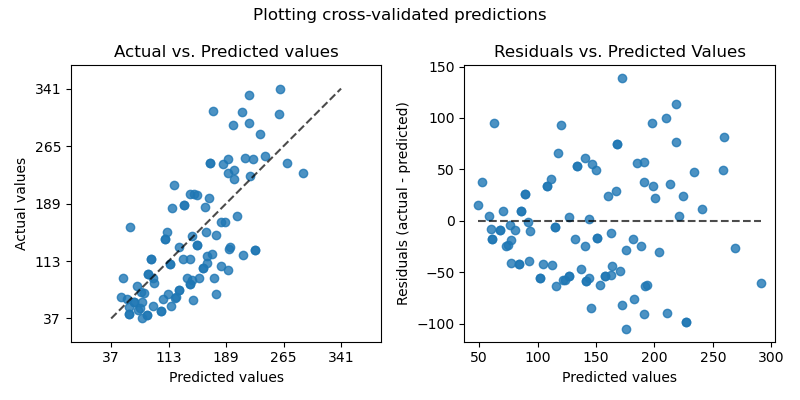
\includegraphics[width = .8\textwidth]{./figs/residuals.png}
    \end{figure}
    \nonumbernote{\tiny from scikit-learn docs}
\end{frame}

\begin{frame}{And in Machine(/Deep) Learning ??}
    \centering
    How many parameters to have\\
    \textbf{Shrek learning botany starting from random noise ?}
\end{frame}

\begin{frame}{And in Machine(/Deep) Learning ??}
    \centering
        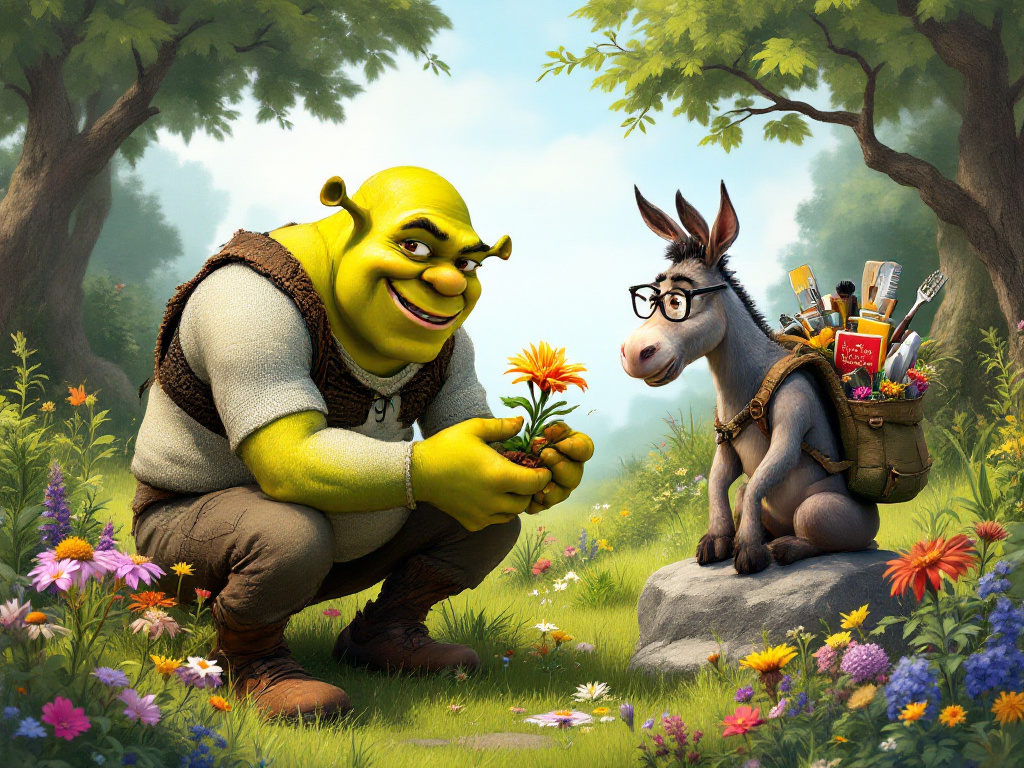
\includegraphics[width = .5\textwidth]{./figs/shrek.jpg}

        $\approx 2.5B$ ?
\end{frame}

\begin{frame}{And in Machine(/Deep) Learning ??}
    \centering
    \textbf{Need to be very carefull on how to evaluate}
\end{frame}

\section{Common traps (in Ecology)}

\begin{frame}{}
    
\end{frame}

\begin{frame}{}
    
\end{frame}

\begin{frame}{}
    
\end{frame}

\section{How to sample and evaluate ?}

\begin{frame}{}
    
\end{frame}



\begin{frame}{Usefull ressources}

\begin{itemize}
    \item \texttt{scikit-learn} docs !
    \item 
    \item 
\end{itemize}
\end{frame}

\begin{frame}[plain]
    \Huge{\textbf{Thanks for you attention !}}
    
    \vfill
    
    \LARGE{\textbf{Let's practice !}}
\end{frame}

\appendix
\begin{frame}[allowframebreaks]{References}
\setbeamertemplate{bibliography item}{}
    {\footnotesize \printbibliography[heading=none]}
\end{frame}


\end{document}
